\section{Extra Features: Quality of Life and Advanced Rulesets}
\label{sec:extra}

To advance beyond the bare-minimum grade cap (Section~3 of the CO2008 specification), the project implements a cohesive runtime configuration system controlled by entering \code{0} at the starting-square prompt. Nine boolean option words (\code{opt\_pretty} through \code{opt\_replay}) occupy contiguous 4-byte slots starting at label \code{options}, allowing the menu loop (\code{src/main.asm}, lines~615--619) to toggle any setting $k \in [1, 9]$ in five branchless instructions: \code{addi \$t0, \$s0, -1; sll \$t0, \$t0, 2; lw \$t1, options(\$t0); xori \$t1, \$t1, 1; sw \$t1, options(\$t0)}. Table~\ref{tab:extra_summary} maps every implemented extension to the specification.

\begin{table}[H]
\centering
\caption{Complete catalog of implemented Quality-of-Life and Advanced Ruleset extensions.}
\label{tab:extra_summary}
\renewcommand{\arraystretch}{1.18}
\rowcolors{2}{rowshade}{white}
\footnotesize
\begin{tabularx}{\textwidth}{c >{\raggedright\arraybackslash}p{3.0cm} >{\raggedright\arraybackslash}p{1.2cm} >{\raggedright\arraybackslash}X}
\toprule
\rowcolor{hcmutlight}
Menu & Option / Action & Spec & Architectural Implementation \& User Rationale \\
\midrule
1 & Pretty Board (default ON) & Sec.~3.1 & Dual-panel ASCII frame with side-by-side square numbers, live piece counts, and active rule banner (\code{print\_board\_pretty}, \code{print\_board\_rules}). \\
2 & Rotate Red (std.\ numbers) & Sec.~3.1 & Rotates board $180^\circ$ during Red's turn via \code{view\_index} ($63 - i$) while retaining canonical square numbers (Spec Fig.~11). \\
3 & Red's Own Numbers & Sec.~3.1 & Applies involution $s' = 33 - s$ in \code{view\_square} and automatically activates board rotation in \code{board\_rotated} so Red's bottom-left is square~29. \\
4 & Detailed Error Messages & Sec.~3.1 & Indexes 12-entry pointer table \code{err\_table} using \code{\$v1} (\code{ERR\_RANGE}..\code{ERR\_BLOCKED}) and rejects invalid starting squares early. \\
5 & Move Hints & Sec.~3.1 & Lists all legal movable pieces (\code{print\_movable\_pieces}) and legal landing squares (\code{print\_landing\_squares}) in active player's numbering, respecting forced capture and chain lock. \\
6 & Forced Capture Rule & Sec.~3.2 & Enforces full English checkers mandatory first capture via \code{side\_has\_capture} inside \code{validate\_move} (returns \code{ERR\_MUST\_CAPTURE}). \\
7 & Flying Kings Variant & Sec.~3.2 & Enables arbitrary-distance diagonal king movement and long-range single-enemy capture (\code{classify\_flying}, \code{can\_capture\_skip}). \\
8 & MARS Bitmap Display & Sec.~3.1+ & Renders $64\times 64$ hardware-style RGB framebuffer at heap \code{0x10040000} with pixel-art pieces and gold king crowns (\code{draw\_bitmap}). \\
9 & Ask to Play Again & Sec.~3.1 & Prompts after victory or agreed draw to restart seamlessly without exiting MARS (\code{main\_game\_over}). \\
10 & Show Move History & Sec.~3.1+ & Prints full match transcript in standard notation (\code{21-17}, \code{14x23 23x32}) from packed 4-byte \code{history[1000]} buffer. \\
11 & Offer / Accept Draw & Sec.~3.1 & Two-phase mutual draw protocol via \code{draw\_offer}; opponent accepts via menu~11 or declines automatically upon making any move. \\
12 & Restart Game & Sec.~3.1 & Resets board, turn, draw state, and move history immediately via \code{new\_game}. \\
13 & Quit & Sec.~3.1 & Clean exit (\code{RESULT\_QUIT} $\to$ \code{syscall 10}) with farewell message. \\
14 & Enable QoL Bundle & Sec.~3.1+ & One-key preset enabling options 1--5 and 9 simultaneously without altering rule variants (6, 7) or Bitmap Display (8). \\
\bottomrule
\end{tabularx}
\end{table}

\subsection{Display Enhancements, Board Rotation, and Player-Relative Numbering}
\label{sec:qol_display}
In standard terminal mode, the raw 8-line grid (\code{\_ r \_ r ...}) forces players to mentally track square indices $1 \dots 32$ and piece tallies. Setting \code{opt\_pretty = 1} (the default whenever \code{pa classic} is omitted) renders:
\begin{itemize}
    \item an active rule header (\code{Kings Standard/Flying | First capture Optional/Required}),
    \item live piece counts computed via \code{count\_pieces(SIDE\_BLACK)} and \code{count\_pieces(SIDE\_RED)}, plus a \code{[Red's view]} badge when rotated,
    \item two synchronized $8\times 8$ bordered grids placed side-by-side: \code{POSITION} (using \code{.} for empty dark squares and spaces for light squares to maximize visual contrast) and \code{PLAYABLE SQUARES} showing the exact square numbers matching the current player's input numbering, and
    \item a concise footer reminding the player that \code{0} opens Settings.
\end{itemize}
Notice how \code{board\_rotated} couples options~2 and~3 cleanly: \code{opt\_rotate | opt\_relnum} is ANDed with \code{side} (\code{0} for Black, \code{1} for Red). Thus, enabling option~3 alone guarantees that Red's board is rotated $180^\circ$ so that Red's bottom-left square is always \code{29}, and during a chain capture \code{play\_turn\_captured} prints \code{"Continue with the piece on square <view\_square(s1, side)>."} so the prompt agrees with the numbers on screen.

\subsection{Move Hints, Detailed Diagnostics, History, Draw Protocol, and Replay}
\label{sec:qol_gameplay}
\begin{itemize}
    \item \textbf{Detailed Error Diagnostics (\code{opt\_detail}):} Every validation failure sets \code{\$v1} to one of 11 symbolic error codes (\code{ERR\_RANGE = 1} through \code{ERR\_BLOCKED = 11}). \code{print\_error} shifts \code{\$a0} left by 2 bits to fetch the matching explanation string from \code{err\_table} in $O(1)$ time, outputting messages such as \emph{``Not a valid move! Pawns can only move forward; only kings move backward. Try again.''}
    \item \textbf{Legal Move Hints (\code{opt\_hints}):} Before the starting-square prompt, \code{print\_movable\_pieces} alerts the player if a forced capture is active and lists all movable squares in player-relative ascending order ($1 \dots 32$). After a valid starting square is entered, \code{print\_landing\_squares} prints all legal destinations (or \code{"none - choose another piece."} and re-prompts without forcing a wasted landing input). During chain captures, \code{print\_landing\_squares} passes \code{\$a2 = 1} to validate exclusively through \code{validate\_chain}.
    \item \textbf{Standard-Notation Move History (Menu 10):} Each executed step packs four bytes into the array \code{history[4*k]}: canonical \code{from}, canonical \code{to}, \code{flags} (bit~0: capture, bit~1: chain step), and \code{side}. \code{print\_history} formats multi-jump chains onto a single numbered line (e.g., \code{8. Red 14x23 23x32}), matching Specification Section~1.3 even when Red played using relative square numbers.
    \item \textbf{Mutual Draw Protocol (Menu 11):} \code{draw\_offer} starts at \code{-1}. When side $p$ chooses~11, \code{draw\_offer} becomes $p$; on the opponent's next turn, \code{notify\_draw\_offer} alerts them to accept via menu~11 (\code{RESULT\_DRAW}) or decline implicitly by playing any legal move (\code{decline\_draw\_offer} resets \code{draw\_offer = -1}). Repeating menu~11 on the offering side prints \code{"You have already offered a draw."} rather than self-accepting.
\end{itemize}

\subsection{Hardware-Style Rendering: MARS Bitmap Display (\code{0x10040000})}
\label{sec:bitmap}
Beyond text UI, \code{draw\_bitmap} (\code{src/board\_io.asm}, lines~576--697) drives MARS's memory-mapped \textbf{Bitmap Display} peripheral directly in the heap segment (\code{BITMAP\_BASE = 0x10040000}). Configured with \code{Unit Width = 8}, \code{Unit Height = 8}, and \code{Display Width/Height = 512}, the display maps a $64 \times 64$ grid of 32-bit \code{0x00RRGGBB} pixel words (16,384 bytes total) onto an $8 \times 8$ tile board where each tile is an $8 \times 8$ pixel sprite.

In production v2.0, \code{draw\_bitmap} combines four microarchitectural optimizations while remaining a \textbf{strict leaf procedure} (zero nested \code{jal} calls):
\begin{enumerate}
    \item \textbf{Dirty-tile caching (\code{bmp\_cache[64]}):} Tracks the last rendered character for all 64 display tiles plus \code{bmp\_valid} and \code{bmp\_last\_rot}. Unchanged tiles skip rendering completely, reducing per-move work from 64 tiles to just 2--3 modified tiles (forcing a full 64-tile redraw on startup, game restart via \code{init\_board}, or $180^\circ$ rotation flip).
    \item \textbf{Loop-Invariant Code Motion (LICM) + pointer stride:} Computes each dirty tile's base framebuffer pointer \code{\$t4} once per tile:
    \begin{equation}
        \text{tile\_base}(r, c) = \texttt{0x10040000} + 4 \cdot \big((r \ll 9) + (c \ll 3)\big),
    \end{equation}
    then strides $+4$\,B per pixel and $+224$\,B per tile row instead of recomputing 2D shifts 64 times per tile.
    \item \textbf{8-way unrolled solid-tile fast path (\code{draw\_bitmap\_solid\_y}):} Empty dark squares and light squares bypass \code{piece\_mask} entirely, emitting 8 consecutive \code{sw \$s2, 0..28(\$t4)} writes per row with stride $+256$\,B/row.
    \item \textbf{Zero-stall load-use scheduling:} Advances the sequential sprite pointer (\code{addi \$t5, \$t5, 1}) immediately inside the load delay slot of \code{lbu \$t3, 0(\$t5)} before \code{beqz \$t3, draw\_bitmap\_put}.
\end{enumerate}
An 8$\times$8 byte sprite mask \code{piece\_mask} encodes \code{0} (background tile), \code{1} (octagonal piece body), and \code{2} (embedded pixel-art crown rendered in gold \code{0x00F1C972} only when \code{\$s4 == 1}, i.e., for kings \code{'B'}/\code{'R'}). Figure~\ref{fig:bitmaps} presents both the $8\times 8$ sprite mask geometry and three pixel-exact live MARS 4.5 captures reconstructed directly from heap dumps (\code{dump 0x10040000-0x10044000 HexText}).

\begin{figure}[H]
\centering
\begin{subfigure}[b]{0.22\textwidth}
    \centering
    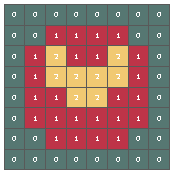
\includegraphics[width=\textwidth]{figures/fig_bmp_mask.pdf}
    \caption{\code{piece\_mask[64]}}
    \label{fig:bmp_mask}
\end{subfigure}
\hfill
\begin{subfigure}[b]{0.24\textwidth}
    \centering
    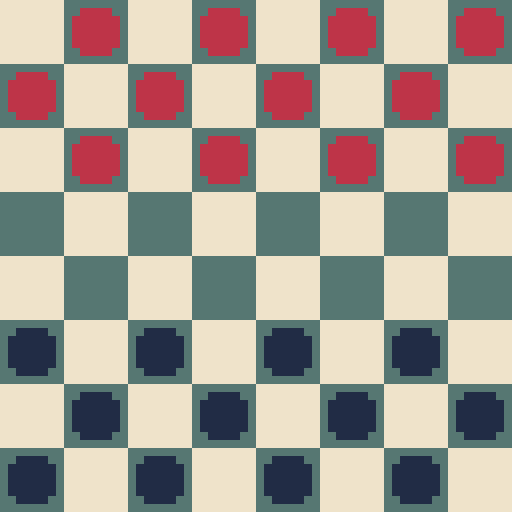
\includegraphics[width=\textwidth]{figures/bitmap_initial.png}
    \caption{Initial (Black's view)}
    \label{fig:bmp_init}
\end{subfigure}
\hfill
\begin{subfigure}[b]{0.24\textwidth}
    \centering
    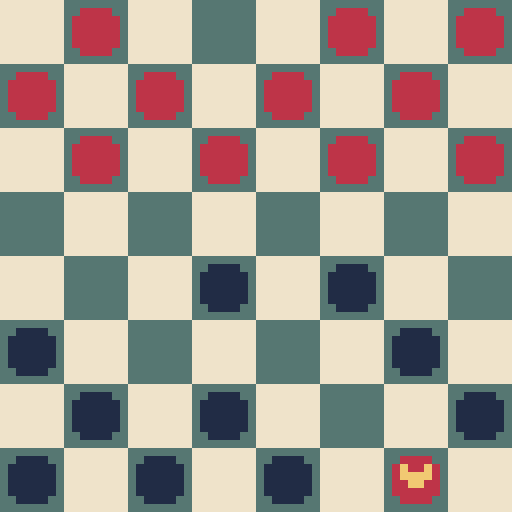
\includegraphics[width=\textwidth]{figures/bitmap_flying_king_setup.png}
    \caption{Red king at sq.\ 32}
    \label{fig:bmp_king}
\end{subfigure}
\hfill
\begin{subfigure}[b]{0.24\textwidth}
    \centering
    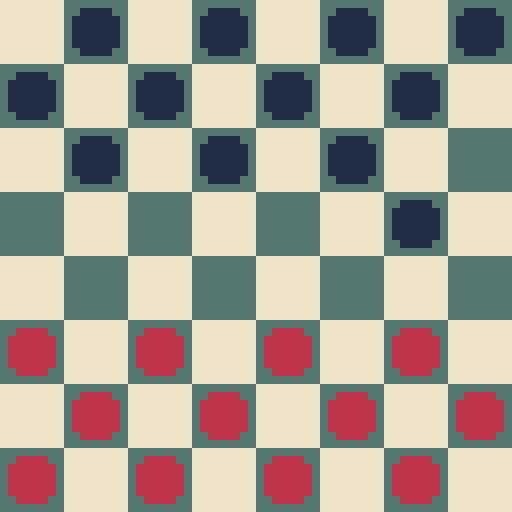
\includegraphics[width=\textwidth]{figures/bitmap_red_rotated.png}
    \caption{Red's $180^\circ$ view}
    \label{fig:bmp_rot}
\end{subfigure}
\caption{Hardware-style MARS Bitmap Display (\code{0x10040000}--\code{0x10043FFF}): (a) 8$\times$8 byte sprite mask (\code{0}=tile \code{\#567772}, \code{1}=body \code{\#BE3448}/\code{\#212C45}, \code{2}=crown \code{\#F1C972}); (b)--(d) live MARS 4.5 framebuffer dumps showing opening setup, gold-crowned Red king ready for flying capture \code{32x14}, and Red's $180^\circ$-rotated board after \code{21-17}.}
\label{fig:bitmaps}
\end{figure}

\subsection{Advanced Rulesets: Forced Capture and Flying Kings}
\label{sec:advanced}
\paragraph{Forced First Capture (\code{opt\_forced}, Menu 6).}
The bare-minimum specification relaxes English Checkers Rule~1 (optional first capture) while keeping Rule~2 (mandatory chain capture). Turning on \code{opt\_forced} restores full tournament English capture obligation: inside \code{validate\_move}, any geometrically valid \code{STEP} triggers \code{side\_has\_capture(side)}, which packs the 32 dark squares into bitboards (\code{BP}, \code{RP}, \code{K}) and evaluates all four diagonal capture directions in parallel via \code{swar\_up\_caps}/\code{swar\_dn\_caps} (falling back strictly to the sparse king bitmask \code{OWN \& K} only when \code{opt\_flying = 1} and no short capture exists). If any capture exists, the non-capturing step is rejected with \code{ERR\_MUST\_CAPTURE}.

\paragraph{Flying Kings Variant (\code{opt\_flying}, Menu 7).}
When \code{opt\_flying = 1} and \code{is\_king} holds, two routines switch from fixed distance $1/2$ to variable-ray diagonal traversal:
\begin{itemize}
    \item \textbf{\code{classify\_flying} (\code{src/rules.asm}, lines~204--229):} Walks intermediate diagonal squares $k = 1 \dots n-1$ between start $s$ and empty destination $d$. Friendly pieces immediately return \code{ERR\_BLOCKED}; enemy pieces increment counter \code{\$s7}, rejecting with \code{ERR\_BLOCKED} if $\$s7 > 1$. Reaching $k = n$ yields \code{STEP} when $\$s7 = 0$ and \code{CAPTURE} when $\$s7 = 1$.
    \item \textbf{\code{can\_capture\_skip} (\code{src/rules.asm}, lines~332--340):} Along each of the four diagonals, skips consecutive \code{EMPTY} squares until hitting a non-empty cell (or off-board \code{0}), then tests whether that cell is an enemy piece with an \code{EMPTY} square immediately behind it.
\end{itemize}
Because \code{do\_move} clears every intermediate cell along the diagonal stride $8\cdot\text{sdr} + \text{sdc}$, flying-king captures remove the jumped enemy automatically regardless of how far before or behind the enemy the king starts or lands.
